\section{Results}\label{sec:results}

\begin{table*}[t]
  \centering
  \caption{\textbf{Identity carried by the state token's key, by readout, in all \nModels{} models.} Second column: key share $s_K = \bar d_K/(\bar d_K+\bar d_V)$ of the answer log-odds under the \fmtOpt{} readout of \citet{anonymous2026fitted}, with 95\% percentile core-bootstrap CIs (10,000 resamples). Remaining columns: $\mathrm{ID}_K$ in nats (the double difference against a third location absent from the story; \cref{sec:method}) under each readout, point estimates. Keys are clamped from layer 0. $n = 150$ story cores per readout and model. The preregistered CI-based tests on these quantities are in \cref{app:prereg}.}
  \label{tab:natural}
  \resizebox{\textwidth}{!}{\begin{tabular}{lcccccc}
\toprule
Model & key share (P1) & \multicolumn{5}{c}{identity carried by keys (nats)} \\
\cmidrule(lr){3-7}
 & & lettered & options after & re-mention & none & options before \\
\midrule
Qwen2.5-1.5B & 0.37 [0.36, 0.39] & +3.6 & +2.8 & -0.5 & +0.2 & -0.2 \\
Qwen2.5-3B & 0.69 [0.68, 0.71] & +11.4 & +10.3 & -0.0 & +0.1 & -0.5 \\
Mistral-7B & 0.92 [0.90, 0.93] & +15.2 & +14.9 & +7.9 & +0.6 & +0.0 \\
OLMo-2-7B & 0.73 [0.71, 0.74] & +7.9 & +8.2 & +2.0 & +0.4 & -0.3 \\
Qwen2.5-7B & 0.82 [0.81, 0.83] & +20.4 & +21.2 & +5.5 & +1.0 & -0.1 \\
Qwen3-8B & 0.84 [0.83, 0.84] & +33.9 & +35.4 & +8.8 & +1.2 & -0.3 \\
Qwen2.5-14B & 0.91 [0.90, 0.91] & +34.8 & +39.0 & +12.1 & +1.1 & -0.1 \\
Mistral-24B & 0.78 [0.77, 0.79] & +9.2 & +9.6 & +5.6 & +0.4 & -0.5 \\
Qwen2.5-32B & 0.86 [0.85, 0.87] & +34.8 & +32.4 & +10.3 & +1.1 & -0.4 \\
Qwen2.5-72B & 0.76 [0.75, 0.77] & +26.4 & +25.6 & +8.4 & +0.5 & -2.0 \\
\bottomrule
\end{tabular}
}
\end{table*}

All quantities are defined in \cref{sec:method}. \Cref{tab:natural} gives the natural key/value factorial for every model and readout, and \cref{fig:formats,fig:scale} summarise it; \cref{fig:localisation} localises the key read at Qwen2.5-1.5B; \cref{tab:frames,fig:frames} revisit the intervention of \citet{anonymous2026fitted}.

\subsection{Re-mentions read the state through the key}\label{sec:res-remention}

\begin{figure}[t]
  \centering
  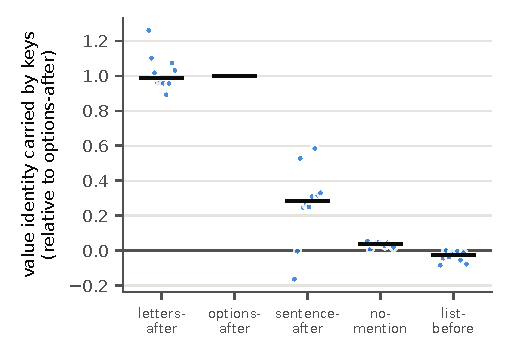
\includegraphics[width=\columnwidth]{figures/fig_formats.pdf}
  \caption{\textbf{Keys carry substantial state identity only when candidates are re-mentioned after the state token.} Identity carried by keys, $\mathrm{ID}_K$, under each readout, divided by its \fmtOpt{} value in the same model. Each dot is one of the \nModels{} models ($n = 150$ story cores per readout and model); horizontal bars are medians across models. Point estimates; absolute values are in \cref{tab:natural}, and the verdicts of the preregistered CI-based tests are in \cref{app:prereg}.}
  \label{fig:formats}
\end{figure}

The readouts fall into three regimes (\cref{tab:natural,fig:formats}).

\textbf{Candidates listed after the state token.} Under \fmtOpt{} and \fmtLetter{}, $\mathrm{ID}_K$ is large and positive in all \nModels{} models, from \idKOptQwenOnefive{} nats at Qwen2.5-1.5B to \idKOptQwenFourteen{} nats at Qwen2.5-14B under \fmtOpt{}. The two option formats give similar values within each model (e.g.\ \idKOptQwenSeven{} and \idKLetterQwenSeven{} nats at Qwen2.5-7B).

\textbf{No reader after the state token.} Under \fmtBefore{}, $\mathrm{ID}_K$ is never above \beforeMax{} nats in any model and is negative in most (down to $\idKBeforeQwenSeventytwo$ nats at Qwen2.5-72B). This is the structural control. The prompt names the same six candidates as \fmtOpt{}, but they precede the state token, so under the causal mask they cannot attend to it. The key effect under \fmtOpt{} therefore depends on whether the candidates appear after the state token, not merely on whether the prompt contains them (the two arms also differ in the answer instruction; \cref{app:prompts}). Under \fmtNone{}, $\mathrm{ID}_K$ is at most \noneMax{} nats, less than a tenth of the \fmtOpt{} value in every model. It is small but not zero: in several models from 7B up it lies outside the $\pm 1$-nat equivalence margin that preregistration A set at 1.5B, which we report as an unpredicted observation (\cref{app:prereg}). In this regime the location is copied mainly from the value (\todo{add $\mathrm{ID}_V$ under \fmtNone{} as macros from the result summaries and cite them here}).

\textbf{A neutral re-mention.} \fmtPost{} names all six locations in a plain sentence after the story and asks for a free-form answer. At Qwen2.5-1.5B and 3B it carries no positive key identity ($\idKPostQwenOnefive$ nats at 1.5B, slightly but reliably negative, and about 0 at 3B). From 7B upward it carries an intermediate amount, from \idKPostOlmoSeven{} nats at OLMo-2-7B to \idKPostQwenFourteen{} at Qwen2.5-14B, between about a quarter and a little over half of the \fmtOpt{} value in the same model. This was not preregistered, and it contradicts the account we held at the time, although it matches the hypothesis we started from (\cref{app:prereg}). After the first 1.5B runs we had narrowed the account, post hoc, to ``listed answer options only''. That narrowed account passed a preregistered fresh-seed test in the same model (preregistration A, $n = 40$ new cores; all three predictions met: $\mathrm{ID}_K$ +2.85 [2.38, 3.33] under \fmtOpt{} and +4.10 [3.45, 4.77] under \fmtLetter{}, CIs inside $\pm 1$ nat under \fmtNone{}, \fmtBefore{} and \fmtPost{}, $s_K$ 0.38 [0.35, 0.41]). It does not generalise. From 7B upward, the neutral re-mention sentence we tested also opens the key channel in every model, and an options list opens it further. This revised account was itself formed after seeing the stage-1 data; preregistration D tests it only in part (\cref{app:prereg}).

\textbf{Preregistered verdicts.} In the five out-of-sample models of stage~1 (Qwen2.5-3B and 7B, Qwen3-8B, Mistral-7B, OLMo-2-7B), $\mathrm{ID}_K > 0$ with a CI excluding 0 under both \fmtOpt{} and \fmtLetter{} (prediction~1), and the paired \fmtOpt{}$-$\fmtNone{} difference is positive with a CI excluding 0 (prediction~2), in 5/5 models each. As part of C4, a \fmtBefore{} control ($\mathrm{ID}_K \leq 0.5$ nats) was preregistered for Mistral-24B, Qwen2.5-32B and Qwen2.5-72B, and it is met in all three ($-0.53$, $-0.42$, $-1.99$). Full scoring is in \cref{app:prereg}.

\subsection{Scale and model families}\label{sec:res-scale}

\begin{figure}[t]
  \centering
  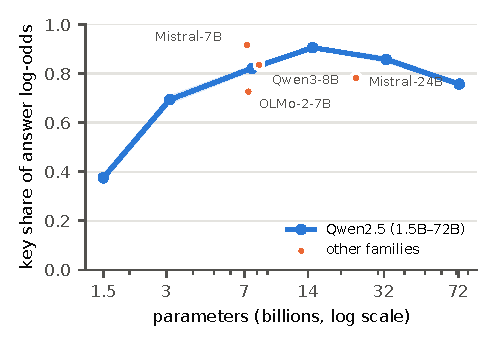
\includegraphics[width=\columnwidth]{figures/fig_scale.pdf}
  \caption{\textbf{Key share of the multiple-choice answer across scale and families.} Key share $s_K = \bar d_K/(\bar d_K+\bar d_V)$ of the answer log-odds under the \fmtOpt{} readout, keys and values clamped from layer 0. Blue line: Qwen2.5-Instruct 1.5B--72B, with 95\% percentile core-bootstrap CIs (10,000 resamples) as the band; orange points: other families. $n = 150$ story cores per model. Values are in \cref{tab:natural}.}
  \label{fig:scale}
\end{figure}

Within Qwen2.5, the \fmtOpt{} key share rises from \shareQwenOnefive{} [\shareLoQwenOnefive{}, \shareHiQwenOnefive{}] at 1.5B through \shareQwenThree{} (3B) and \shareQwenSeven{} (7B) to \shareQwenFourteen{} [\shareLoQwenFourteen{}, \shareHiQwenFourteen{}] at 14B, and then falls to \shareQwenThirtytwo{} at 32B and \shareQwenSeventytwo{} [\shareLoQwenSeventytwo{}, \shareHiQwenSeventytwo{}] at 72B (\cref{fig:scale}). The curve is non-monotonic: the 14B and 72B intervals do not overlap. $\mathrm{ID}_K$ under \fmtOpt{} has the same shape (\cref{tab:natural}). The depth-matched clamp onset ($l_0 = 0.0625\,L$) gives the same shares to two decimals in every Qwen2.5 model, and nearly identical shares in the other families. The other families fall in a similar range: Qwen3-8B \shareQwenThreeEight{}, Mistral-7B \shareMistralSeven{}, Mistral-24B \shareMistralTwentyfour{} and OLMo-2-7B \shareOlmoSeven{}. Every model except Qwen2.5-1.5B puts more than half of the multiple-choice effect in the key.

The key-share part of the preregistered prediction C4, $s_K \geq 0.80$ at each of Mistral-24B, Qwen2.5-32B and Qwen2.5-72B, is not met: the threshold holds only at Qwen2.5-32B (\cref{app:prereg}). We do not know why the share falls beyond 14B. The large-model shares are close to those implied by our reanalysis of the fixed-value experiment of \citet{anonymous2026fitted}, which, from 1-based block~6 onward, fixes the critical-token values to the target run's, restores the recipient's attention outputs through that token and varies the keys: \sKQwenFV{} at Qwen2.5-72B (ours: \shareQwenSeventytwo{}) and \sKMistralFV{} at Mistral-24B (ours: \shareMistralTwentyfour{}). The two are different estimands, so we read this only as agreement in magnitude.

\subsection{The option words are the readers}\label{sec:res-readers}

\begin{figure}[t]
  \centering
  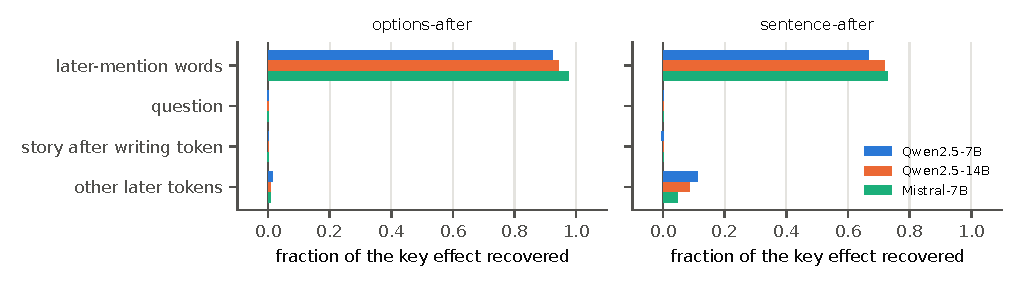
\includegraphics[width=\columnwidth]{figures/fig_localisation.pdf}
  \caption{\textbf{The re-mentioned option words read the key.} Exact row-restricted key swap at Qwen2.5-1.5B: only the listed token group sees the source key at the state token, at every layer, while all other rows see the base key. Bars give the fraction of the full key effect (all rows see the source key) that this recovers, as a ratio of mean log-odds changes over $n = 40$ story cores; point estimates. Blue: \fmtOpt{}; orange: \fmtLetter{}.}
  \label{fig:localisation}
\end{figure}

To find which later tokens read the state token's key (an exploratory analysis; localisation at scale is preregistered as D3), we let only one group of rows see the source key, using the exact row-restricted splice (\cref{sec:method}), at Qwen2.5-1.5B (\cref{fig:localisation}). The six option words recover \locOptChoicewords{} of the full key effect under \fmtOpt{} and \locLetterChoicewords{} under \fmtLetter{}. Every other group recovers between $\locOptStorytail$ and \locLetterQuestion{} in both formats: the question rows, the story after the state token, and the remaining rows (instruction, chat template, prefill and answer position). The remaining rows, including the answer position, therefore gain nothing from seeing the source key themselves. This is consistent with the key changing what the option words retrieve and the answer then reading the option words, although we did not test the second step directly. Restricting the swap further by layer and KV group, the read happens in layers 4--15 of 28 and one of the two KV groups dominates (\cref{app:additional}). An exploratory attention probe, run in an earlier prompt configuration, agrees: with the source key in place, the option word that matches the key's location attends to the state token, as it does in the source run (\cref{app:additional}).

Because \fmtPost{} carries no key identity at 1.5B, the corresponding question for the neutral re-mention can only be asked at scale. \todo{Stage 3 (preregistration D, prediction D3): row-restricted localisation at Qwen2.5-7B, Qwen2.5-14B and Mistral-7B ($n = 60$) under \fmtOpt{}, \fmtLetter{} and \fmtPost{}, including re-mention-word rows under \fmtPost{}, plus layer-window and KV-group localisation. Report met/not met.}

\subsection{Generality across tasks}\label{sec:res-tasks}

We test whether the same regimes hold for two further state-writing tasks, repainting an object and rescheduling it to a day, in five 7--14B models (preregistration D). \todo{Stage 3: $\mathrm{ID}_K$ under all readouts, \fmtOpt{}$-$\fmtNone{} contrasts and \fmtBefore{} control for the paint and schedule tasks; verdicts for D1 and D2.}

\subsection{Revisiting a learned remap: behaviour transfers, key carriage does not}\label{sec:res-paper1}

\begin{figure*}[t]
  \centering
  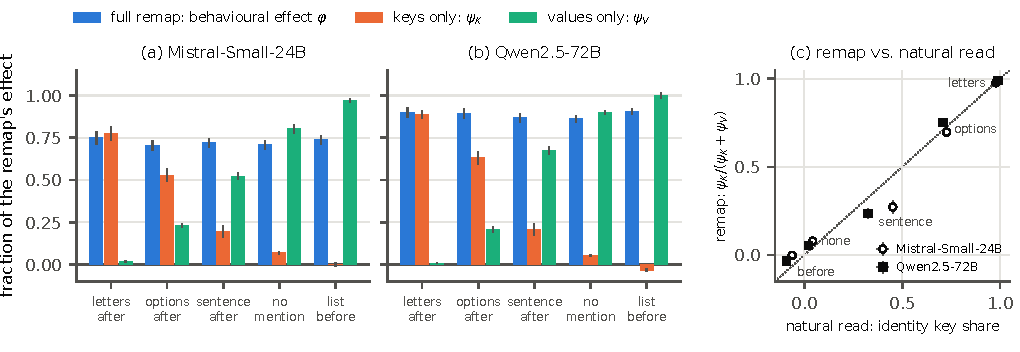
\includegraphics[width=\textwidth]{figures/fig_frames.pdf}
  \caption{\textbf{The learned remap of \citet{anonymous2026fitted} changes behaviour almost equally under every readout, but its attribution to critical-token keys is large only when candidates are listed after the state token, and weak with a neutral re-mention.} Released rank-16 bases (seeds 101--103) at Mistral-Small-24B (left) and Qwen2.5-72B (right). Blue: $\varphi$, the learned remap's shift relative to the PCA patch, as a fraction of the natural source-to-target shift. Orange: $\psi$, the fraction of the learned--PCA difference produced by giving the PCA run the learned run's critical-token keys. Green (values printed): $\rho$, the fraction removed by giving the learned run the PCA run's keys. Keys are exchanged from 1-based block~6 on, as in \citet{anonymous2026fitted}; queries and values evolve. $n = 96$ native story cores with base, source and target distinct; fits averaged within core. Error bars: 95\% core-bootstrap CIs (10,000 resamples). Values in \cref{tab:frames}.}
  \label{fig:frames}
\end{figure*}

\begin{table}[t]
  \centering
  \caption{\textbf{The intervention of \citet{anonymous2026fitted} under five readouts.} Point estimates with 95\% core-bootstrap CIs (10,000 resamples) over $n = 96$ native story cores with base, source and target distinct; the three released fits are averaged within core. $\varphi$: full learned remap; $\psi$: key-only addition (learned keys into the PCA run); $\rho$: key-only removal (PCA keys into the learned run). The options-after row (\fmtOpt{}) is the readout of \citet{anonymous2026fitted}.}
  \label{tab:frames}
  \resizebox{\columnwidth}{!}{\begin{tabular}{llccc}
\toprule
Model & Format & $\varphi$ (full remap) & $\psi$ (key addition) & $\rho$ (key removal) \\
\midrule
Mistral-Small-24B & lettered options & 0.75 [0.71, 0.79] & 0.78 [0.73, 0.82] & 0.99 [0.98, 0.99] \\
 & options after & 0.70 [0.68, 0.73] & 0.53 [0.49, 0.56] & 0.76 [0.75, 0.78] \\
 & re-mention sentence & 0.72 [0.69, 0.75] & 0.20 [0.16, 0.23] & 0.45 [0.43, 0.47] \\
 & no re-mention & 0.71 [0.68, 0.73] & 0.07 [0.06, 0.08] & 0.18 [0.16, 0.20] \\
 & options before & 0.74 [0.71, 0.76] & -0.00 [-0.01, 0.01] & 0.01 [-0.00, 0.02] \\
\midrule
Qwen2.5-72B & lettered options & 0.90 [0.87, 0.93] & 0.89 [0.86, 0.91] & 0.99 [0.99, 1.00] \\
 & options after & 0.89 [0.86, 0.92] & 0.63 [0.59, 0.67] & 0.79 [0.78, 0.81] \\
 & re-mention sentence & 0.87 [0.84, 0.89] & 0.21 [0.17, 0.24] & 0.34 [0.31, 0.36] \\
 & no re-mention & 0.86 [0.84, 0.88] & 0.05 [0.05, 0.06] & 0.11 [0.09, 0.12] \\
 & options before & 0.91 [0.89, 0.92] & -0.03 [-0.04, -0.02] & -0.02 [-0.04, -0.01] \\
\bottomrule
\end{tabular}
}
\end{table}

\citet{anonymous2026fitted} find that critical-token keys contribute causally to the behavioural difference between their learned remap and an unfitted PCA patch, scoring the direct location question, whose readout lists the candidates after the question, together with two observer colour-lookup questions. We revisit the direct location question only. We first reproduce their setting item by item: with their released bases, encoder and pinned model revisions, the argmax answers of the learned (M) and PCA (P) runs under \fmtOpt{} agree with their saved outputs on 0.994--1.000 of core--fit items (Mistral-24B: M 0.994, P 1.000; Qwen2.5-72B: both 1.000; $n = 360$ each), which passes the preregistered 0.95 gate. We then change only the readout (\cref{tab:frames,fig:frames}). Apart from C2 and C3, the comparisons across readouts below are exploratory in preregistration C. Unlike \citet{anonymous2026fitted}, who score argmax agreement, we report fractions of log-odds effects.

\textbf{Behaviour is nearly readout-invariant.} Relative to the PCA patch, the learned remap moves the answer by nearly the same fraction of the natural source-to-target shift in every format: $\varphi$ lies between \phiOptMistral{} and \phiLetterMistral{} at Mistral-24B and between \phiNoneQwen{} and \phiBeforeQwen{} at Qwen2.5-72B. The PCA patch transfers the source location at a rate of 1.00 in every format.

\textbf{Key carriage is not.} Giving the PCA run the learned run's keys reproduces \psiLetterQwen{} of the learned--PCA difference under \fmtLetter{} and \psiOptQwen{} under \fmtOpt{} at Qwen2.5-72B, but only \psiPostQwen{} under \fmtPost{}, \psiNoneQwen{} under \fmtNone{}, and $\psiBeforeQwen$ under \fmtBefore{}. Mistral-24B follows the same order (\psiLetterMistral{}, \psiOptMistral{}, \psiPostMistral{}, \psiNoneMistral{}, about 0). Removal behaves the same way: replacing the learned run's keys with the PCA run's undoes \rhoLetterQwen{} of the difference under \fmtLetter{} but \rhoNoneQwen{} under \fmtNone{} and $\rhoBeforeQwen$ under \fmtBefore{} (Qwen2.5-72B; Mistral-24B \rhoLetterMistral{}, \rhoNoneMistral{}, \rhoBeforeMistral{}). The preregistered prediction C3, $\psi_{\fmtNone{}} < 0.5\,\psi_{\fmtOpt{}}$, is met in both models.

Taken together, under \fmtNone{} the learned run keeps most of its effect without its own critical-token keys, so the edit must reach the answer by another route: plausibly the critical-token value, although we exchanged neither values nor other event-span positions. Under \fmtLetter{} the keys alone are sufficient for most of it and necessary for nearly all of it. One reading, formed after seeing these data and not preregistered, is that the remap writes its edit into both channels and the readout decides which channel is read; $\varphi$ varies little across formats, which is consistent with this. On the direct location question, the key result of \citet{anonymous2026fitted} holds under their readout ($\psi = \psiOptQwen{}$, $\rho = \rhoOptQwen{}$ at Qwen2.5-72B), but how much of the edit the keys carry depends on the readout, not only on the intervention. We did not re-test their colour-lookup questions.

\subsection{Preregistered transfer-law predictions that failed}\label{sec:res-failed}

Before stage~2 we preregistered a transfer law (C1): the learned remap's free-form effect $\varphi_{\fmtNone{}}$ should lie within $\pm 0.15$ of its value-channel completeness $\kappa_V$, estimated beforehand from the fixed-value clamping data of \citet{anonymous2026fitted}. It fails at Mistral-24B: predicted 0.53 $\pm$ 0.15, observed \phiNoneMistral{} [\phiLoNoneMistral{}, \phiHiNoneMistral{}]. At Qwen2.5-72B it is met only at the edge of the margin: predicted 0.73 $\pm$ 0.15, observed \phiNoneQwen{} [\phiLoNoneQwen{}, \phiHiNoneQwen{}]. The companion prediction C2, that the remap transfers less to free-form answers than to the multiple-choice format of \citet{anonymous2026fitted} ($\varphi_{\fmtOpt{}} - \varphi_{\fmtNone{}} > 0$), is not met at Mistral-24B ($-0.003$ [$-0.019$, $+0.013$]) and is met, but small, at Qwen2.5-72B ($+0.034$ [$+0.018$, $+0.049$]).

In both models the observed free-form effect exceeds $\kappa_V$: beyond the margin at Mistral-24B, and near its upper edge at Qwen2.5-72B. One reading, formed after seeing these data, is that the value channel carries the remap more fully than the fixed-value estimate implied. Here, completeness measured by clamping one channel to another run's state, under one readout, did not predict how the intervention transfers to another readout. We have no tested explanation for the gap. Together with the C4 threshold (\cref{sec:res-scale}), the post hoc options-only account and the \fmtNone{} identity outside the $\pm 1$-nat margin at scale (\cref{sec:res-remention}), this is one of several places where our expectations failed; all preregistered outcomes are listed in \cref{app:prereg}.
